\chapter{Leveraging Symmetry}
\label{ch:symmetry}

One obvious path towards faster-and-better learning relies on exploiting the motion symmetry
that is a common attribute of human and animal locomotion;
gait symmetry is an indicator of healthy outcomes in 
physiotherapy~\citep{robinson1987use, riskowski}.
Relatedly, while asymmetric gaits are often associated 
with physical injuries and neural impairments such as stroke.  
A symmetry constraint or symmetry-favoring bias thus offers a readily available and convenient 
path towards faster learning and more realistic outcomes. 
It is also largely orthogonal to most other efficiency improvements.

Naively, exploiting symmetry might be expected to yield a $2\times$ learning speedup, and may help to avoid
some of the undesired asymmetric local minima that \ac{DRL} is prone to exploit.  On the other hand,
it could also be the case that asymmetric policies and motions serve a useful role as an intermediate path 
towards finding eventual optimal symmetric motions, and therefore
hard symmetry constraints may in fact be problematic.
Another important subtlety is that while a symmetric policy is helpful in achieving symmetric motions,
it does not guarantee a symmetric outcome.
For example, a quadruped gallop and a biped lope are asymmetric gait cycles, 
as each gait cycle begins with a leading left or right foot, while the underlying 
policy can still be fully symmetric.

What is the best way to integrate a symmetry bias or other forms of symmetry enforcement into the learning process?
How much benefit does it really offer in terms of learning speed and learning outcomes?
What are other considerations for symmetry-informed methods?
The principle contribution our work is an in-depth analysis and comparison of four different methods
of incorporating symmetry into the learning process:
\begin{description}
\item [DUP]  Duplicating tuples with their symmetric counterpart.
\item [NET]  Enforcing symmetry in the network itself.
\item [LOSS] Adding a symmetry auxiliary loss.
\item [PHASE] Motion phase mirroring.
\end{description}
Two of these methods are new (DUP,NET) and two are already present in existing literature (LOSS, PHASE), 
albeit without a systematic evaluation of all the issues around symmetry enforcement. 
The methods incorporate knowledge of symmetry into the policy structure (NET), 
the learning data (DUP, PHASE), or via the learning loss (LOSS). 
We also believe that the results are of more general interest, because they 
illustrate (and experimentally validate) various ways that inductive biases 
can be incorporated into \ac{DRL} methods.

\section{Symmetry Enforcement Methods}
\label{sec:methods}
We now describe four different methods for enforcing symmetry, using duplicate tuples, auxiliary losses, 
a time-indexed motion phase, and architecture-based methods.  
We begin by first formally defining symmetric trajectories and symmetric policies.  
Two trajectories are symmetric if for each state-action tuple, $(s,a)$, from one trajectory, 
the corresponding state-action tuple is given by $(\mathcal{M}_s(s), \mathcal{M}_a(a))$ 
for the other trajectory, where $\mathcal{M}_s$ and $\mathcal{M}_a$ are defined as follows,

\begin{align*}
    &M_s: \mathcal{S} \to \mathcal{S} &  &M_a: \mathcal{A} \to \mathcal{A}\\
    &M_s(s) = \text{the mirror of state } s & &M_a(a) = \text{the mirror of action } a\\
\end{align*}

Note that the mirroring functions are attributes of the environment, and
not attributes of the enforcement method or learning pipeline.  Here we use {\em environment}
to refer to combination of the character, it's simulated world, and the task, as is common
in RL settings.
All the symmetry enforcement methods we shall describe
require both of these functions as a minimal requirement.  
Similarly, we can define a symmetric policy to be one where the following holds
% \autoref{eq:symmetric-policy} holds 
for all states $s \in \mathcal{S}$:

\begin{align}
    \pi_\theta(M_s(s)) = M_a(\pi_\theta(s)).
    \label{eq:symmetric-policy}
\end{align}

A symmetric policy thus produces the mirrored action when given the mirrored state as input. 
RL methods such as PPO also use state-value functions during the learning process.  
The output of these value functions should remain unchanged for any state and its mirrored counterpart.  
The construction of the mirror functions for our environments (\autoref{sec:environments}) are further 
elaborated in \autoref{sec:mirroring-functions}.

The methods discussed in this section attempt to achieve symmetric gaits by encouraging or constraining 
the learned policies to be symmetric. However, even if successful, this may be insufficient to guarantee a symmetric gait.  
In particular, a symmetric policy may learn to favor motions with staggered poses, where a given dominant foot is always in front.
This may confer advantages with respect to balance and agility.  
Once  such a policy is initialized to an initial asymmetric staggered pose, it can continue
with an asymmetric motion.
With regard to the policy, it is not always possible to achieve exact symmetry in a parameterized model 
such as a neural network.  For example, regions of the state space may remain unexplored 
during the learning process, and thus symmetry cannot be enforced for such regions.  
Therefore, the equality in \autoref{eq:symmetric-policy} is not always assumed to be strict.

It is possible to directly optimize for gait symmetry with reinforcement learning by 
including quantitative symmetry measures in the reward function, such as the Symmetry Index~\citep{robinson1987use} 
or other possible measures~\citep{symmetry_measures}. However, we share the sentiment 
of previous work~\citep{Yu-SIGGRAPH-2018} that directly optimizing such measures 
may be ineffective, as they introduce delayed or sparse rewards that may make the learning problem more difficult.  
Consequently, our work focuses on methods that can be used for obtaining approximately 
symmetric policies, which are described in the remainder of this section.

% Before all else, we start by making clear what we mean by symmetry by making a distinction. Importantly, by symmetry here we do not refer to \textit{invariance} to mirroring, rather the notion is closer to \textit{equivariance}. A policy that is invariant to mirroring will output the same action whether the state is mirrored or not, but in our case if the state is mirrored the action should be mirrored as well. Although, in this case the value function should be invariant to mirroring in the state instead.

% \gre{note on difference of state and observation and why I'm using state here?}

%Let us assume that $\phi(s_t) = \phi(s_{t'}) + 0.5$. Then in this scheme an auxiliary reward $r_{sym} = -d(s_t, s_{t'})$ could be added to the existing reward function where $d$ is a distance function between states.

\subsection{Duplicate Tuples (DUP)}
\label{subsec:dup_epx}
This method may be the most intuitive way for achieving symmetry and is a form of data augmentation.  
In this approach each trajectory tuple is duplicated and mirrored, and is then
added as a valid experience tuple along with the original.  
More formally, let $\tau=(s_1, a_1, r_1, \dots, s_T)$ 
be a trajectory sampled from the environment.  
A post-processing step will compute the mirrored trajectory of $\tau$, 
i.e.\ $\tau' = \left( M_s(s_1), M_a(a_1), r_1, \dots, M_s(s_T) \right)$, and both $\tau$ and $\tau'$ 
will be added to the roll-out memory buffer for learning.  
Notice that the rewards, $r_1, \dots, r_{T-1}$ are the same in both $\tau$ and $\tau'$.  
This is because the reward function $r(s, a)$ is automorphic under the symmetry transformation, namely 
$r(s, a) = r(\mathcal{M}_s(s), \mathcal{M}_a(a))$.

One drawback of using this approach is that the mirrored tuples are not strictly on-policy,
as assumed by policy-gradient RL methods. Thus it could be problematic when used with methods 
such as PPO~\citep{ppo} and TRPO~\citep{trpo}.  
The off-policy issue arises because at training time the policy $\pi_\theta$ is not guaranteed 
to be symmetric, and therefore the probability of sampling action $M_a(a_t)$ from $\pi_\theta(M_s(s_t))$ 
may be really low, effectively corresponding to an off-policy action.
However, our results show that this is not necessarily a critical issue in practice.

\subsection{Auxiliary Loss (LOSS)}
In this method proposed by~\citeauthor{Yu-SIGGRAPH-2018}\cite{Yu-SIGGRAPH-2018}, 
the authors create a symmetry loss defined as follows:
\begin{align}
L_{sym}(\theta) = \sum_{t=1}^{T} \norm{ \pi_\theta(s_t) - M_a ( \pi_\theta( M_s(s_t) ) ) }^2
\end{align}
and optimize this as an auxiliary loss in addition to the default PPO loss:
\begin{align}
\pi_\theta = \argmin {\theta} L_{PPO}(\theta) + w L_{sym}(\theta),
\end{align}
where $w$ is a scalar hyper-parameter used to balance the gait symmetry loss
with the standard policy optimization loss which aims to maximize the original objective. 
The authors use $w=4$ for their results. 
An alternative approach would be to simply include the symmetry loss as an extra reward term. 
However, the auxiliary loss is generally preferable;
the loss term is differentiable and therefore provides a clear signal to optimize 
rather than being included via the PPO-approximated gradient.  
Changing the reward function may also induce unexpected behaviors.

The authors in \cite{Yu-SIGGRAPH-2018} show improvements in the sample efficiency for their 4 tasks with a 
factor of approximately two (see Figure~8 in \cite{Yu-SIGGRAPH-2018}).
%Interestingly, the symmetric loss does not seem to be helpful at the start of the training and only.
However, the symmetric loss is shown to be beneficial only in the context of a given curriculum learning algorithm;
in its absence, there was no significant improvement over a vanilla-PPO baseline,
and in one case (the humanoid) using the symmetric loss proved to be detrimental (please refer to the same plot).
The addition of an extra hyper-parameter may generally be seen as undesirable. 
However, in practice we find in our experiments that the method is not very sensitive 
to the choice of $w$ and we end up using the default value in all settings.

\subsection{Phase-Based Mirroring (PHASE)}

To study locomotion, the gait can usually be divided into repeated \textit{gait cycles},
which can then further be parameterized using a phase variable $\phi \in [0,1)$,
which then wraps back to $\phi=0$ upon reaching $\phi=1$.
A common assumption is to advance the phase linearly with time.  
Another strategy that can help provide additional robustness is to perform a
phase-reset at each bipedal foot strike, e.g., set $\phi=0$ upon left-foot strike
and $\phi=0.5$ upon right foot strike. 
To enforce symmetry, a policy is only learned for the first half cycle, 
and is replaced by the policy with mirrored states-and-actions during the second half cycle:
\begin{align}
    a_t = \begin{cases}
    \pi_\theta(s_t) & 0 \leq \phi(s_t) < 0.5\\
    M_a(\pi_\theta(M_s(s_t))) & 0.5 \leq \phi(s_t) < 1
    \end{cases}
    \label{eq:phase-based-symmetry}
\end{align}

In our experiments, we strictly advance the motion phase as a function
of time and we do not implement phase-resets.  For forward-progress tasks,
this then corresponds to providing a mandated duration for each half-cycle of the motion.
The phase-based method is particularly useful for imitation-guided learning scenarios
such as those presented in~\cite{2017-TOG-deepLoco},~\cite{2018-TOG-deepMimic},
and~\cite{cassie-sim-to-real}.
The goal in these cases is to imitate a reference motion capture clip with 
the help of a phase-indexed reward that measures the distance from the reference motion.
The use of the PHASE symmetry in that context is motivated by the potential
for faster learning.

The PHASE approach is simple to implement and does not require modifying training in any way 
since it can be implemented directly within the environment. 
However, the potential for abrupt changes exists at $\phi=0.5$ when the 
phase is strictly computed as a function of time.

\subsection{Symmetric Network Architecture (NET)}

\begin{figure}%
  \centering
  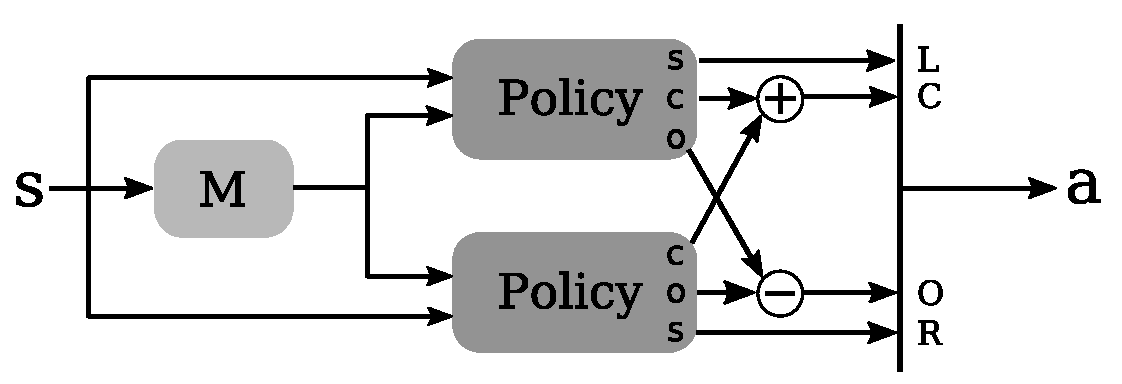
\includegraphics[width=0.9\columnwidth]{symmetry_figures/net_architecture_2.pdf}
  \caption{A universal method for converting any neural network into a symmetric network policy.}{$\mathcal{M}$ block is an environment-dependent state mirroring function. The two policy blocks are the same neural network module, with the output terminals re-order for illustration clarity.  The \textit{s, c, o} terminals corresponds to \textit{side}, \textit{common}, and \textit{opposite} joints as described in \autoref{sec:mirroring-functions}.}
  \label{fig:net-architecture}
\end{figure}

Another approach towards enforcing symmetry is to impose symmetry at the network architecture level. 
The goal here is to choose a network architecture such that \autoref{eq:symmetric-policy} 
holds for all states~$s$ and all network parameters~$\theta$.
There are multiple ways to go about designing such an architecture.
However they may require some knowledge about how the actions and/or states 
in which case having access to the mirroring functions $M_s$ and $M_a$ is strictly-speaking not enough.

A general case description of this method would be lengthy, and thus we focus only on the key aspects here. 
The simplest case occurs when we can assume that the action vector is simply divided 
into two, one corresponding to each side of the body, 
and that the actions of one side can readily be applied to the other side through a simple swapping operation.
This ignores the common parts such as the torso and the head for the time being.
More concretely, consider:
\begin{align*}
    a &= \begin{bmatrix}a_l\\a_r\end{bmatrix} \\
    M_a(a) &= \begin{bmatrix}a_r\\a_l\end{bmatrix}
\end{align*}
where $a_l$ and $a_r$ are vectors of equal size.
In this case we can define a symmetric policy composed of an inner network $f$ as follows:
\begin{align*}
    \pi_{side}(s) = \begin{bmatrix}
    f(s,M_s(s))\\
    f(M_s(s),s)\\
    \end{bmatrix}
\end{align*}
It is easy to show in this case that \autoref{eq:symmetric-policy} holds:
\begin{align*}
    \pi_{side}(M_s(s)) &= \begin{bmatrix}
    f(M_s(s),M_s(M_s(s)))\\
    f(M_s(M_s(s)),M_s(s))\\
    \end{bmatrix}\\
    &= \begin{bmatrix}
    f(M_s(s),s)\\
    f(s,M_s(s))\\
    \end{bmatrix}\\
    &= M_a\left( \begin{bmatrix}
    f(s,M_s(s))\\
    f(M_s(s),s)\\
    \end{bmatrix} \right)\\
    &= M_a\left(\pi_{side}(s)\right)
\end{align*}

When the action space also includes actions for common parts,
i.e., those such as the torso and head that have no symmetric counterparts,
it is easy to define $\pi_{com}(s) = h(s) + h(M_s(s))$ 
which is then invariant to left/right mirroring. 
Finally, the policy is then a combination of the common actions and the side actions:
\begin{align*}
    \pi_\theta(s) = \begin{bmatrix}
        \pi_{com}(s)\\
        \pi_{side}(s)\\
    \end{bmatrix}
\end{align*}
Please refer to \autoref{fig:net-architecture} for an illustration of the NET method.

A drawback of this method is that it requires knowledge about the symmetry structure of the actions/states 
and that it needs to redefine the network structure. 
Also, this method is highly sensitive to state/action normalization.
The problem is that an ordinary normalization based on the past experiences may break the symmetry.
Though the other methods introduced here can also suffer from the same problem, this method is much more sensitive to the issue.

\subsection{Practical Considerations}

There are a number of practical considerations to take into account when working with 
each of the methods introduced in previous section.
In terms of implementation, the DUP and PHASE methods are the easiest to 
implement as they required little to no change to the learning pipeline.  
Architecture-based mirroring (NET)
requires the most modification to both the learning pipeline and the environments.
The LOSS method is the only approach here that allows us to balance the desire for symmetry 
with the original learning objective, albeit at the cost of an extra hyper-parameter.  
The NET method produces a truly symmetric policy, which is not possible with the other methods.
The PHASE method is the approach best suited for coping with neutral states, 
which represent symmetric states where it may become problematic to break symmetry.
We revisit this point later.
PHASE is also restrictive in that it enforces a predefined walk cycle timing.

%% normalization 

One more consideration relates to the application of normalization to network inputs, which is commonly done by 
using statistics gathered from the data itself.  
However, this can break some of the mirroring assumptions.  
The problem is most severe when using a symmetric network architecture, although other methods are
also impacted.
Fortunately, developing a normalization scheme that works correctly is relatively straightforward. 
A simple approach is to duplicate the states (or actions) as in \autoref{subsec:dup_epx} 
and to compute the statistics based on the aggregated set of states (or actions) and 
their mirrored states (or actions).



\section{Gait Symmetry Metrics}

All of the methods discussed only provide indirect paths, via the learned policies, 
for achieving symmetry for the actual motions. 
Therefore it is important to evaluate how well these methods do at achieving their final goal. 
\citeauthor{Yu-SIGGRAPH-2018}\cite{Yu-SIGGRAPH-2018} use an established metric in the biomechanics literature 
known as the Robinson Symmetry Index (SI):
\begin{align}
    SI = \frac{2|X_R - X_L|}{X_L + X_R}\cdot 100,
\end{align}
where $X_R$ is a scalar features of interest, such as the duration of the stance phase 
for the right leg, and $X_L$ is its counterpart for the left leg. 
Previous work using the LOSS method~\cite{Yu-SIGGRAPH-2018} chooses to use the average actuation 
magnitude as the parameter of interest which leads to $X_R = \sum_{t=1}^T \norm{\boldsymbol{\tau}_{t,R}}_2$ where $\boldsymbol{\tau}_{t,R}$ is the vector of applied torques at time $t$ for the right leg. 
We will refer to this as the \textit{actuation symmetry index (ASI)}.
In practice we found that the ASI can be misleading in some circumstances, 
e.g., With this metric a high torque applied to the right hip can be conflated with a high torque applied to the left knee, 
which is not desirable. ASI also loses information about signs of the applied torques.

The \textit{phase-portrait} is another tool that can be used to qualitatively investigate 
the symmetry or asymmetry of a gait, as seen in \cite{symmetry_phase_portrait}. 
The phase-portrait is a scatter plot drawn over a period of time, usually over a single gait cycle.
The $x$ and $y$-axes of the 2D plot correspond to the position and velocity, respectively, of a joint of interest, 
such as the hip flexion, 
For an asymmetric gait the phase portraits of the two sides will not fully overlap.
To numerically quantify the similarity between two phase-portraits, we propose to use a~\textit{phase-portrait index} (PPI).  
One problem to address is that the left and right limbs usually have a phase offset even for a symmetric motion.
This is not a problem when inspecting the phase-portraits visually, but the problem needs to be addressed to compute a 
meaningful metric.
We solve this by finding the best phase offset between the left and the right side through an exhaustive search. 
We also normalize each axis so that $x,y\in[-1,1]$ to address the potential discrepancy between magnitudes of different gaits.
The final PPI is defined according to:
\begin{align}
    PPI = \frac{1}{C} \min_s \sum_{t=0}^{C-1} \norm{q_t^R - q_{t+s}^L}_1 + \norm{\dot{q}_t^R - \dot{q}_{t+s}^L}_1,
\end{align}
where $C$ is the length of a gait cycle, $q_t^R$ and $\dot{q}_t^R$ are the normalized right joint 
position and velocity at time $t$. Similarly, $q_{t+s}^L$ is the normalized left joint position 
at time $t+s$ modulo $C$, as the elements that are shifted beyond the last position are reintroduced at the beginning.

\section{Environments}
\label{sec:environments}
\begin{figure}%
  \centering
  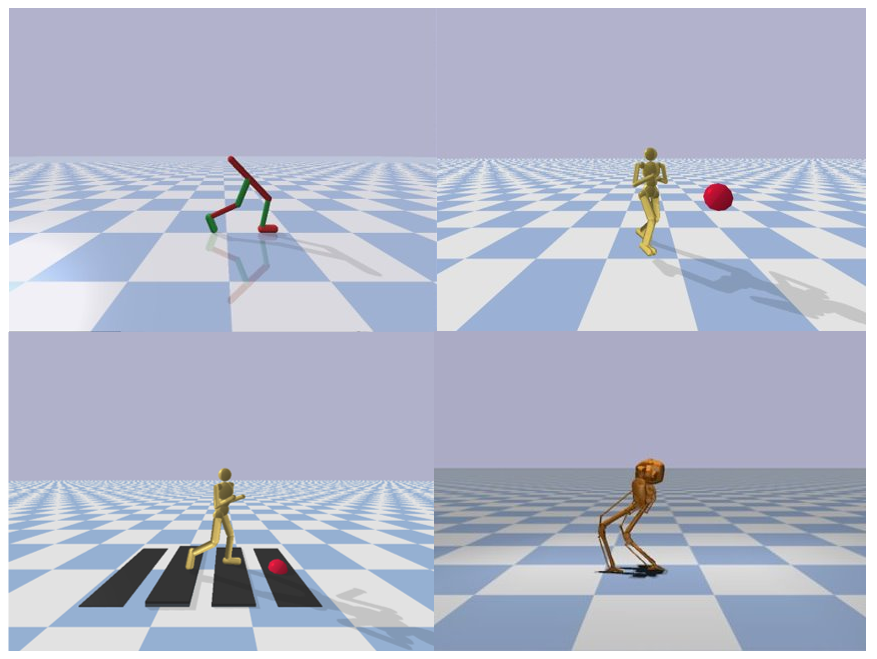
\includegraphics[width=0.9\columnwidth]{symmetry_figures/task_overview_2.png}
  \caption{Environments.}{Top-left: {\it Walker2D}. Top-right: {\it Walker3D}. Bottom-left: {\it Stepper}. Bottom-right: {\it Cassie}.}
  \label{fig:task-overview}
\end{figure}

We evaluate the effectiveness of the enforcement methods described in \autoref{sec:methods} 
on four different locomotion taks, i.e., RL ``environments''.  
The environments were chosen to represent a fairly diverse range of locomotion tasks.  
They are described in detail below.  
For each environment, we run each method 5 times and plot the mean results.

\bfpara{Walker2D}  The implementation of {\it Walker2D} environment is taken directly from PyBullet \citep{ref:Pybullet} 
without further modification.  The purpose of this environment is to evaluate each symmetry method on 
a well-established existing reinforcement learning environment.  
The task is for the character to walk as far as possible in the forward direction in the allotted time.  
An action is a 6D vector corresponding to a normalized torque at each of the hip, knee, and ankle on both left and right legs.  
The observation space is~22D and consists of root information (root z-coordinate, x and y heading vector, root velocity, 
roll, and pitch), joint angles, joint angular velocities, and binary foot contact information.

\bfpara{Walker3D}  This represents a 3D character simulated in PyBullet, with targets randomly placed, at a distance,
in the half-plane in front of the character.  
The task requires character to navigate towards the target and then stop at the target.  
A new target will be chosen, in the forward half-plane of the current character orientation, 
once the target is reached and one second has passed.  
The 3D character has 21-DoF corresponding to abdomen (x3), hip (x3), knee, ankle, shoulder (x3), and elbow.  
The observation space is 52D, and is analogous to that provided for {\it Walker2D},
with an additional 2D vector representing the target location in the character root frame.

\bfpara{Stepper}  The {\it Stepper} environment uses the same model as \textit{Walker3D}, and 
requires it to navigate terrain consisting of a sequence of stepping blocks.  
The blocks are randomly generated with the following statistics, as sampled from their respective distributions:
spacing $d \sim \mathcal{U}(0.65, 0.85)$ meters and height variation of the next step $h \sim \mathcal{U}(0, 25)^{\circ}$.  
The character receives information for two upcoming blocks as an $(x,y,z)$ offset in character root space.  
The stepping block information advances when either foot contacts the immediate next block, 
which effectively forces character to step precisely on each step.  
The precise foot placement requirement, as well as variable terrain height, makes this environment 
more challenging than \textit{Walker3D}.

\bfpara{Cassie}  The task requires a bipedal robot Cassie to walk forward at a desired speed 
while mimicking a reference motion.  Since the reference motion is time indexed, the character receives a phase variable as input.  
The phase variable varies according to $\phi \in [0,1)$ in the gait cycle.  
In addition to phase, the character receives other inputs including the height, the orientation expressed as a unit quaternion,
pelvis velocities, angular velocities, and acceleration, joint angles and angular velocities.  
In total, the Cassie robot has a 10D action space and 47D observation space.  
Another important distinction between {\it Cassie} and the other tasks is that it is implemented in 
MuJoCo~\citep{ref:Mujoco}, while other environments use the Pybullet~\citep{ref:Pybullet} physics engine. 
This simulated model has also been validated to be close to the 
physical Cassie robot~\cite{cassie-sim-to-real}.


\section{Results}

We compare the four methods, together with an asymmetric baseline, across four different 
locomotion tasks of varying difficulties.  

\subsection{Summary}

We begin with a high-level summary of our  findings.
All methods of enforcing symmetry constraints have no consistent-and-predictable impact,
positive or negative, on learning speed. This is contrary to our initial expectations. 
However, this does not provide the full picture, as
high-scoring policies can often succeed via unintuitive asymmetric gaits.
There also exist tasks for which the asymmetric baseline simply never succeeds without the
help of symmetry, i.e., Stepper.
Thus symmetry methods should be used to reliably produce higher-quality symmetric motions, 
i.e., closer to what we might expect from human and animal movement.
While the symmetry methods are not all equal, they cannot be reliably ranked in terms of performance.
An exception occurs in imitation-guided task settings, where the reward is related to imitating a
time-indexed reference motion, such as for \textit{Cassie} and \textit{DeepMimic}.
In such cases, the PHASE method appears to be superior in terms of learning speed,
as compared to the asymmetric baseline and the other methods.
We further compare and contrast the different methods in two sections below.

\subsection{Effect on Learning Speed}

One of our initial hypotheses was that the learning speed can be improved by enforcing symmetry.  
Symmetry can be considered as domain knowledge that may otherwise be difficult for to learn, 
especially considering its abstract nature.  
However, our experiments indicated that enforcing symmetry in general has no consistent impact on the learning speed.
As shown in \autoref{fig:learning-curves}, BASE performs well in \textit{Walker2D} and \textit{Walker3D}.  
In particular, although BASE was not initially the fastest in \textit{Walker3D}, 
it ultimately achieves a higher return than all mirroring methods.  
On the other hand, BASE fails to learn the \textit{Stepper} task in all five runs;
it often pauses near the beginning without taking a single step.  
This is consistent with findings by \citeauthor{Yu-SIGGRAPH-2018}, 
who also find that symmetry enforcement can be crucial when learning more difficult tasks.

For the \textit{Cassie} environment, the benefit of enforcing symmetry is evident 
because the reward explicitly encourages the character to imitate a symmetric reference motion.  
We hypothesize that for such a case, symmetry constrains the search space in a suitable way 
for the symmetric task. However, if symmetry is not rewarded, explicitly or implicitly, 
then its effects may not be reflected in the learning curve.  Finally, between the symmetry methods, 
there is no clear winner in terms of learning speed.

\begin{figure*}[tbh]
  \centering
  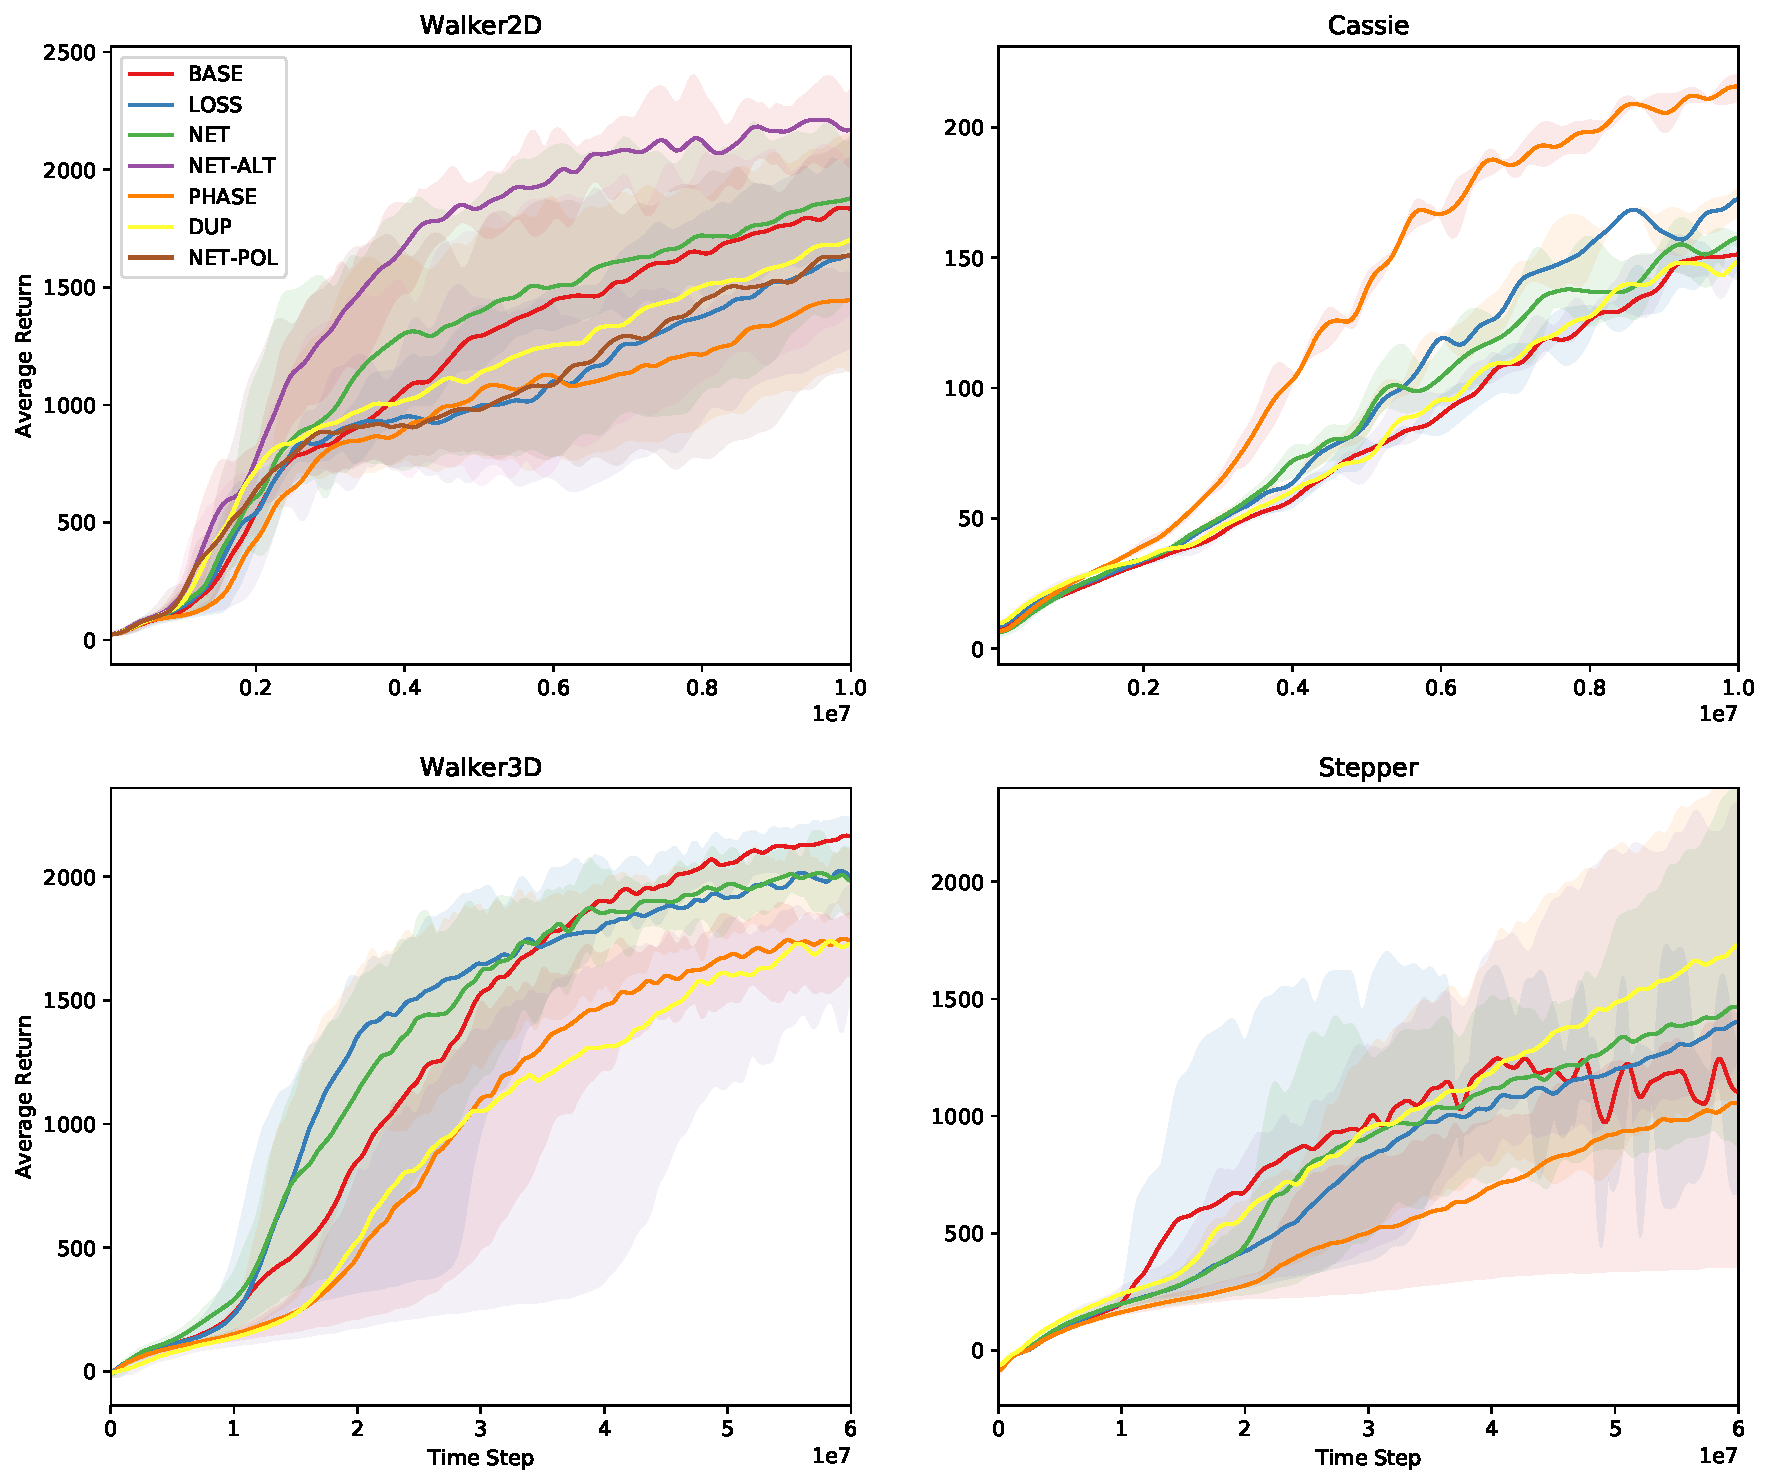
\includegraphics[width=\columnwidth]{symmetry_figures/LearningCurves.pdf}
      \caption{Learning curves for different symmetry methods in each of the four locomotion environments (\autoref{sec:environments}).}{The \textit{Walker2D} plot contains two additional experiments aside from the baseline and four symmetry methods.  \textit{NET-ALT} uses an alternate formulation of symmetric network architecture described in \autoref{sec:alternate-network}.  \textit{NET-POL} is an ablation study on \textit{NET} with symmetry enforcement only on the policy network and not on the value network.}
  \label{fig:learning-curves}
\end{figure*}

\bfpara{PHASE and Imitation-Guided Learning}  In phase-based symmetry experiments, 
we define a phase variable in correspondence to the gait cycle.  
For the \textit{Cassie} environment, we use a period of 0.8~s, 
which is determined based on the reference motion.  
For all other environments, we assign a period based on a working solution.

We find phase-based symmetry enforcement to be effective for imitation-guided learning, 
as it outperforms other methods by a significant margin for \textit{Cassie}.  
When comparing \textit{Cassie} with \textit{DeepMimic}~\cite{2018-TOG-deepMimic}, 
which also uses an imitation objective, we find the results to be consistent.  
The learning curves for our \textit{DeepMimic} symmetry experiment are presented in \autoref{sec:deepmimic-results}.  
We hypothesize that phase-based symmetry is effective for imitation-guided tasks when
the motion clips used for training containing suitably-periodic and symmetric motions.  
On the other hand, PHASE constrains the period of the gait cycle, 
which can be harmful for non-imitation tasks. 
PHASE performs poorly in terms of learning speed 
when used without a reference motion, i.e., 
for \textit{Walker2D}, \textit{Walker3D}, and \textit{Stepper}, although
it can do well in terms of quality, e.g., for \textit{Walker3D}.

\bfpara{Alternate Symmetric Network}  The NET method presented in \autoref{fig:net-architecture} is 
an intuitive way of converting any neural network into a symmetric policy.  
However, it is perhaps not the immediate solution that one would come up with when tasked to design a symmetric neural network.  
We include one of our earlier constructions of symmetric policy in \autoref{sec:alternate-network}, 
which we refer to as NET-ALT.  A major difference between NET and NET-ALT is that the latter uses 
shared weights at the layer level to explicitly enforce the symmetry constraint in \autoref{eq:symmetric-policy}.  
Despite this, the two architecture-based mirroring methods should, in theory, have similar performance.  
As can be seen in \autoref{fig:learning-curves}, NET-ALT significantly outperforms NET in the \textit{Walker2D} environment, 
along with the baseline and all other mirroring methods.  
We believe that the structure of the symmetric layer matrix in \autoref{sec:alternate-network} 
may be the key to resolve this gap, which remains to be verified.

\bfpara{Policy Network Ablation Study}  As an ablation study, we removed the symmetry constraint 
for the value network in the NET method.  Since our goal is to produce a symmetric policy, 
and the value network is discarded after training, we want to see how enforcing symmetry in the value network 
during training affects the learning speed.  In \autoref{fig:learning-curves}, the two curves of interest are 
NET and NET-POL, where the latter has the symmetry constraint removed for the value network.  
Our experiment shows that it is beneficial to enforce the symmetry constraint for the value network during training, 
since the difference between the curves is not insignificant.  

\subsection{Symmetry Enforcement Effectiveness}

Although learning speed is a major point of interest from the ML perspective, 
our work is nevertheless motivated by the aesthetics of symmetric gaits that is needed for applications in animation.  
We measure the effectiveness for each symmetry enforcement methods on the metrics we defined in \autoref{sec:metrics}.  
In most cases, we find that symmetric gaits are better achieved when any of the enforcement methods are applied, 
as compared to the baseline.  The motions produced by the symmetry methods are also more 
natural-looking, subjectively speaking, than without mirroring (see supplementary video). 

The symmetry metrics results are summarized in \autoref{tab:actuation_si} and \autoref{tab:pp_msi}.  
In order to perform consistent measurement for the metrics, we omit the first two strides of data 
in order to limit the influence of the transition period from standing to locomotion.  
The reported metrics are calculated from the median of the ten subsequent strides after the initial two.  
For the \textit{Stepper} tasks, we use median from five strides to accommodate for the increased difficulty.  
Also note the \textit{Stepper} results are missing for BASE because it was unable to produce 
consistent gait cycles that can be measured.  In most cases, the policy either learns to pause 
at the starting location or falls after taking one or two steps.

As in learning speed, there is not a single best mirroring method across all environments.  
However, from the overall picture, we found that LOSS and PHASE to be the most consistent among all methods.  
In general ASI and PPI do not agree on a single best method except for the \textit{Cassie} task where PHASE is the best.


\begin{table}[tbh]
    \centering
    \begin{tabular}{l|c|c|c|c}
    & Walker2D & Walker3D & Stepper & Cassie  \\
    \hline
    BASE & \textit{3.97} & 6.36 & \xmark & 9.27   \\
    DUP & 3.77 & 7.57 & 7.54 & 6.58   \\
    LOSS & 2.56 & 4.48 & 6.36 & \textit{15.72}   \\
    NET & 2.00 & \textit{10.64} & \textit{28.97} & 5.15   \\
    PHASE & 3.77 & \textbf{2.55} & \textbf{3.99} & \textbf{4.49}   \\
    NET-ALT & \textbf{1.04} & -- & -- & --   \\
    NET-POL & 1.71 & -- & -- & --   \\

    \end{tabular}
    \caption{Actuation SI. Lower numbers are better.}
    \label{tab:actuation_si}
\end{table}


\begin{table}[tbh]
    \centering
    \begin{tabular}{l|c|c|c|c}
    & Walker2D & Walker3D & Stepper & Cassie  \\
    \hline
    BASE & \textit{1.06} & \textit{2.16} & \xmark & \textit{0.49}   \\
    DUP & 0.39 & 1.61 & 0.57 & 0.41   \\
    LOSS & 0.33 & \textbf{0.19} & \textbf{0.46} & 0.31   \\
    NET & \textbf{0.16} & 0.58 & \textit{0.65} & 0.23   \\
    PHASE & 0.57 & 0.30 & 0.49 & \textbf{0.17}   \\
    NET-ALT & \textbf{0.16} & -- & -- & --   \\
    NET-POL & 0.28 & -- & -- & --   \\
    \end{tabular}
    \caption{Phase Plot Index. Lower numbers are better.}
    \label{tab:pp_msi}
\end{table}



\section{Discussion}

Symmetry can sometimes be harmful, especially when the character begins from or otherwise arrives at a neutral pose,
i.e., a symmetric pose where $s = M_s(s)$.  The problem is that a symmetric policy is incapable of escaping 
from a neutral pose, since the action that it takes would also be symmetric.  
When a symmetric action is applied in a symmetric state, the next state is necessarily also symmetric.  
For instance, a character that starts from the T-pose will likely perform some kind of hopping gait, 
since the feasible locomotion possibilities which perpetuate symmetric states and actions are limited.  
To make matters worse, states near the neutral states can also become problematic.

The breaking-symmetry problem is most severe when enforcing symmetry through network architecture, as this method is guaranteed to produce true symmetric policies.  While DUP and LOSS methods can suffer from the same issue, they can implement workarounds at an additional cost.  This issue, however, does not affect PHASE.
A simple workaround to this problem is to always start the character from a non-neutral position.  This can be easily achieved by adding some random noise to each joint of the initial pose at the start of the task.  In practice, we did notice that
on occasion the character would converge on a hopping gait. However the simple workaround works well 
for the majority of cases in our experiments.

% \subsection{Is Perfect Symmetry Always Desirable?}

Our work is motivated by the premise that healthy human gaits are usually symmetric.  
However, this still remains a controversial issue in the biomedical literature~\cite{riskowski, SADEGHI200034}.  
The strongest argument for asymmetry in human motor control is the general belief that humans have a dominant side that is often the preferred choice for manipulating objects.  This is also tied with the need for a leading foot to start a walk or run cycle in the neutral state problem.  One should therefore be aware of the implications when enforcing perfect symmetry.
Quadrupedal locomotion, which has six commonly observed gaits as opposed to the three gaits of bipeds \cite{locomotion_mcmahon}, is also interesting to examine.  Of these six, half are fairly symmetric including walk, trot, and rack. However the remaining three, also known as the in-phase gaits which are used at high speeds, are often asymmetric. Since the symmetry of gait and policy are not the same, it would be interesting to see whether it is possible to nevertheless 
achieve these non-symmetric quadrupedal gaits with a symmetric policy.

\section{Conclusions}

In this paper, we explore the use of symmetry constraints for DRL-based learning of locomotion skills.
We compared four different enforcement methods, in addition to a symmetry-free baseline, 
across four different locomotion tasks of varying difficulty.  
We find that enforcing symmetry constraints can in fact sometimes be harmful to learning efficiency,
but that in general it produces higher quality motions.  For some tasks it enables 
When comparing the symmetry methods, we find that the results, both in terms of learning speed and motion symmetry, 
to be environment-dependent.  A notable exception is that the phase-based mirroring method generally 
performs better than the the baseline for imitation-guided reward settings such as for \textit{Cassie} and \textit{DeepMimic}.

The difference between the enforcement methods is more pronounced from the implementation standpoint.  
LOSS and PHASE methods have the burden of an additional hyperparameter to tune. 
However, the additional parameter can also be viewed as an advantage in terms of flexibility.  
In LOSS, the hyperparameter can be used to adjust the strength of symmetry constraint.  
For PHASE, the phase variable allows us to define a desired locomotion period. 
Given the similarities across all methods, it is perhaps justifiable to choose one based on the implementation overhead.  
DUP is the easiest to implement and evaluate since it requires minimal change to 
existing RL pipeline and has no hyperparameter to tune.  
Finally, if the application requires absolute symmetry, then the NET method is guaranteed to produce a symmetric policy.

The application of symmetric policies is not limited to locomotion.  
Many classical control tasks may benefit significantly from leveraging symmetry, 
including acrobat, cart-pole, and pendulum \citep{ref:OpenAI-Gym}.  
Furthermore, the notion of symmetry extends beyond left-right symmetry and even character motion.  
The Sudoku game is an example task that exhibits multiple types of symmetry properties. 
Whether a learning method can take full advantage of all the symmetries remains an open question.
However, this paper lays a foundation for enabling future studies on inductive biases
based on symmetry.